\section{Lattices of Groups.}
\label{section1}

\begin{definition}
    Let $G$ be a group. We define the  \textbf{lattice} of subgroups of $G$ to
    be a directed graph whose set of vertices are subgroups of  $G$, and whose
    edges are given by the relation $(H,K)$ if $H \leq K$, for  $H,K$ subgroups
    of  $G$.
\end{definition}

We detail an algorithm for generating the lattice of subgroups of a given group
$G$.

\begin{algorithm}
    For any group $G$:
    \begin{enumerate}
        \item[\textbf{step 1:}] Plot $G$ and  $\vbrack{e}$ opposite each other.

        \item[\textbf{step 2:}] Plot a gubgroup $H$ of  $G$. If there are no
            subgroups $A$ such that $H \leq A \leq G$, connect  $H$ to  $G$. If
            there are no subgroups $A$ such that  $\vbrack{e} \leq A \leq H$,
            connect $H$ to  $\vbrack{e}$. If there are no subgroups left to
            plot, go to \textbf{step 5}.

        \item[\textbf{step 3:}] For any other subgroup $K$ plotted on the graph,
            if there is no subgroup $A$ such that  $H \leq A \leq K$, or $K \leq
            A \leq H$, then connect  $K$ to  $H$.

        \item[\textbf{step 4:}] return to \textbf{step 2}.

        \item[\textbf{step 5}] return.
    \end{enumerate}
\end{algorithm}

The lattice of subgroups of a group, can also be viewed as a lattice of
partially ordered sets, instead of a graph. We focus however on the graph
theoretic apprach. We now ist numerous examples.

\begin{example}\lable{2.11}
    \begin{enumerate}
        \item[(1)] For $\faktor{\Z}{m\Z}=\vbrack{1}$, we plot the lattice of
            subgroups for $m=2,4,12, p^n$ where $p$ prime and $n \in \Z^+$:
            \begin{figure}[h]
                \centering
                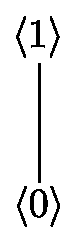
\includegraphics[scale = 0.5]{Figures/Chapter2/Z_2_lattice.eps}
                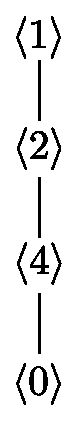
\includegraphics[scale = 0.5]{Figures/Chapter2/Z_8_lattice.eps}
                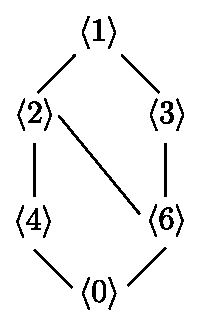
\includegraphics[scale = 0.5]{Figures/Chapter2/Z_12_lattice.eps}
                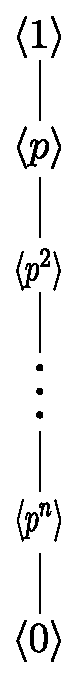
\includegraphics[scale = 0.5]{Figures/Chapter2/Z_p^n_lattice.eps}
                \caption{The lattices of $\faktor{\Z}{2\Z}$, $\faktor{\Z}{8\Z}$,
                $\faktor{\Z}{12\Z}$, and  $\faktor{\Z}{p^n\Z}$ respectively.}
                \label{fig_2.1}
            \end{figure}
            Notice that only the lattice of $\faktor{\Z}{12\Z}$ conatains any
            cycles.

        \item[(2)] The lattice of subgroups of $D_8=\vbrack{r,t}$ is that of
            figure \ref{fig_2.2}
            \begin{figure}[h]
                \centering
                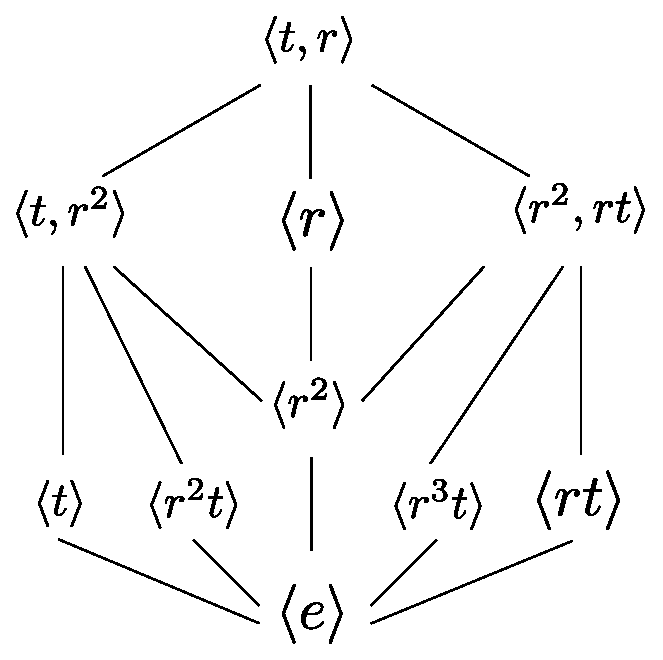
\includegraphics[scale = 0.5]{Figures/Chapter2/D_8_lattice.eps}
                \caption{The lattices of $D_8$.}
                \label{fig_2.2}
            \end{figure}
            This lattice can be drawn as a planar graph, however it is not true
            that all lattices of $D_8$ are planar. The lattice of $D_{16}$
            for example, cannot be drawn as a planar graph.

        \item[3] The lattice of $S_3$ is the attice in figure \ref{fig_2.3}
            \begin{figure}[h]
                \centering
                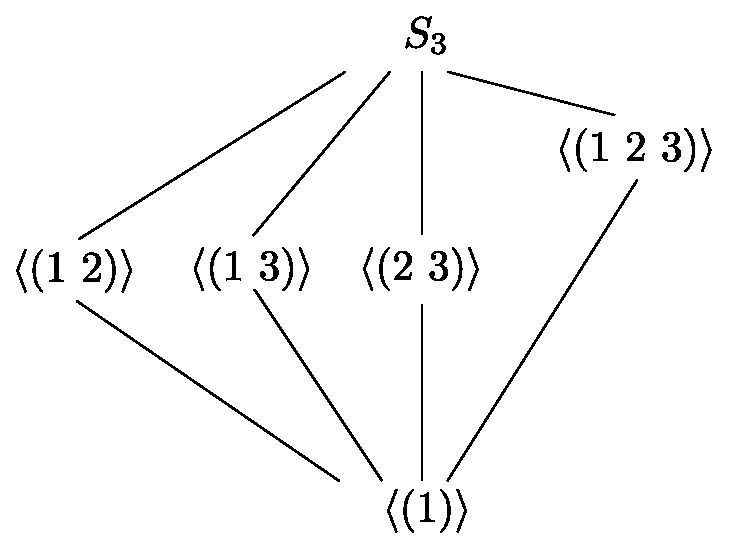
\includegraphics[scale = 0.5]{Figures/Chapter2/S_3_lattice.eps}
                \caption{The lattices of $S_3$.}
                \label{fig_2.3}
            \end{figure}

        \item[(4)] The lattice of $U(\faktor{\Z}{12\Z})$ is that of figure
            \ref{fig_2.4}
            \begin{figure}[h]
                \centering
                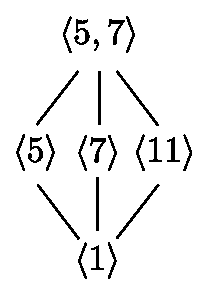
\includegraphics[scale = 0.8]{Figures/Chapter2/U(Z_12)_lattice.eps}
                \caption{The lattices of $U(\faktor{\Z}{12\Z})$.}
                \label{fig_2.4}
            \end{figure}

        \item[(5)] The \textbf{Klein-$4$ group} is the Abelian group $V_4$
            defined by the following Cayley table:
            \begin{equation*}
                \begin{matrix}
                    1 & a & b & c \\
                    a & 1 & c & b \\
                    b & c & 1 & a \\
                    c & b & a & 1 \\
                \end{matrix}
            \end{equation*}
            and has the lattice of figure \ref{fig_2.5}.
            \begin{figure}[h]
                \centering
                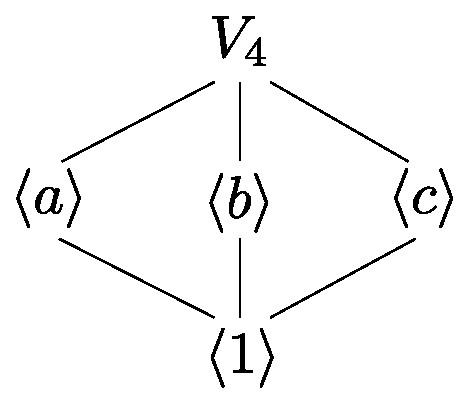
\includegraphics[scale = 0.5]{Figures/Chapter2/V_4_lattice.eps}
                \caption{The lattices of $V_4$.}
                \label{fig_2.5}
            \end{figure}
            Notice that as a graph, the lattice of subgroups of $V_4$ is
            isomorphic to the lattice of subgorups of $U(\faktor{\Z}{12\Z})$.
    \end{enumerate}
\end{example}

These examples provide intereseting notions. The first is the notion of the
``join'' of two subgroups.

\begin{definition}
    For any two distinct subgroups $H$ and $K$ of a group, the \textbf{join} of
    $H$ and  $K$ is the smallest subgroup, $vbrack{H,K}$ containing both  $H$
    and  $K$.
\end{definition}

\begin{lemma}\label{2.5.1}
    Let $H$ and  $K$ be distinct subgroups of a group. Then the join
    $\vbrack{H,K}$ is unique.
\end{lemma}
\begin{proof}
    Supose there exists another smallest subgroup containing $H$ and $K$, and
    call it $A$. Then  $A \subseteq \vbrack{H,K}$. But by definition,
    $\vbrack{H,K}$ is minimal, thus it must be contained in $A$ as well, so
    $\vbrack{H,K} \subseteq A$. This establishes equality, and hence uniqueness.
\end{proof}

\begin{lemma}\label{2.5.2}
    If $G$ and  $H$ are isomorphic groups, then they have the same lattice of
    subgroups.
\end{lemma}
